\documentclass[preview,12pt]{article}
\usepackage{amsmath}
\usepackage{gensymb}
\usepackage{ragged2e}
\usepackage{geometry}
\usepackage{graphicx}
\usepackage{caption}
\usepackage{subcaption}
\usepackage{pdfpages}

\geometry{letterpaper, margin=1in}

\begin{document}

\begin{center}
    \section*{Shadowgraph Visualization of the Effects of a Magnetic Field Applied to a Detonation Wave}
    \textbf{Josh Coffey\footnote{Graduate Research Assistant, Department of Aerospace Engineering, AIAA Student Member}, Vijay Anand\footnote{Senior Researcher, Department of Aerospace Engineering, AIAA Young Member}, Rachel $\textbf{Wiggins}^1$, Ephraim Gutmark\footnote{Professor, Department of Aerospace Engineering, AIAA Fellow}}
    $$\textit{ University of Cincinnati, OH- 45221, USA}$$
\end{center}


\begin{abstract}
    Pulsed detonation combustors (PDCs) are a form of pressure gain combustion that make use of detonations to generate energy.  This is in contrast to traditional combustors that use subsonic deflagrations.  The main advantage of PDC’s is the significant efficiency increases over deflagration based combustion as well as being a simpler design.  In this paper, shadowgraph images are taken of a detonation wave propagating through a clear, polycarbonate detonation tube under the influence of an applied magnetic field.  This allows for a qualitative analysis of the changes caused by the  applied magnetic field to the detonation wave.  In addition, using pressure sensors, the pressure at different points in the tube is measured in order to analyze the changes caused by the magnetic field.
\end{abstract}

\begin{center}
    \section*{\footnotesize{1.  Introduction}}
\end{center}

Detonation based combustors are currently being developed due to their increased thermodynamic efficiency over traditional Brayton cycle based combustors [1].  They are currently being considered for use in everything from earth based power production to rocket engines [1,2].  In the latter, it has been suggested that performance can be improved by including a magnetohydrodynamic (MHD) generator in the system [3,4].  After the detonation wave passes through a region, part of the gas behind the wave is ionized and it has been suggested that an MHD generator be attached to the detonation tube in order to extract energy from the combustor [5,6].  This energy could then be used as electrical power to power the aircraft's subsystems or as a method of increasing aircraft performance [4,6,7].  However, in order for this concept to work, the detonation wave would be required to pass through a relatively powerful magnetic field. 
\newline
\indent The effects of the magnetic field on the detonation wave are described using magnetohydrodynamics, which is the study of electrically conducting fluids [8].  By using the equations that govern MHD effects, the effects of the application of a magnetic field on the moving ionized gas left in the wake of the detonations can be modeled.  When a magnetic field is applied to a moving charge, motional emfs are generated. [17]  This electromotive force can be expressed as: 
\begin{equation}
    \varepsilon=\oint f_{mag}\cdot dl=vBh
\end{equation}
where $f_{mag}$ is the magnetic force per unit charge, $dl$ is around a current loop once the integration is carried out, $v$ is the velocity of the moving charge, $B$ is the magnetic field, and $h$ is the width of the circuit loop which, in this case, is the distance between the walls through which the detonation wave propagates, i.e. the channel width.  In the case of a magnetic dipole, such as a bar magnet centered at the origin and along the z-axis, the magnetic flux density $B$ can be calculated using the equation
\begin{equation}
    \textbf{B}=\frac{\mu_0}{4\pi}\frac{m}{r^3}(2cos\theta\textrm{ }\hat{r}+sin\theta\textrm{ }\hat{\theta})
\end{equation}
This emf induces an electromotive current in the fluid which can be calculated by
\begin{equation}
    \textbf{J}=\sigma(\textbf{E}+\textbf{v}\times \textbf{B})
\end{equation}
where $\sigma$ is the electrical conductivity of the medium. \newline
\indent These effects have been studied in detail in the past, both theoretically and experimentally, and the goal of this study is to attempt to visualize these changes [9-15].  The main driver of any changes to the detonation wave is expected to be the Lorentz force:
\begin{equation}
    F_{Lorentz}=\textbf{E}+\textbf{v}\times\textbf{B}
\end{equation}
\indent According to previous studies, when this force is directed against the detonation wave the velocity of the wave is as much as 10\% less than the Chapman-Jouguet velocity, while there is no effect when the force is in the direction of the wave's propagation [11,16].  Other numerical studies have shown that a transverse magnetic field can also reduce the velocity of the wave [13,15].  In addition, it has been shown numerically that the pressure behind the detonation wave may decrease as a result of a magnetic field [13].  
\newline
\indent It has also been shown that while the magnetic field can have an impact on the detonation wave, the interaction may also affect the magnetic field strength.  According to one study, the magnetic field strength decreases inside the detonation wave and in the area behind the detonation wave where high temperatures cause ionization [9].  
\newline
\indent In addition, it is possible that this study will give greater insight into the decoupling nature of a detonation wave under the influence of a magnetic field.  As the Chapman-Jouguet detonation wave weakens, especially due to the opposing magnetic force, it is expected that the reaction front and lead zone begin to decouple.  It has previously been shown numerically that the amount of decoupling between the reaction front and lead zone is related to the strength of the magnetic field [15].  Because a coupled reaction front and lead zone is necessary for the Chapman-Jouguet wave to propagate, the decoupling behavior is of interest [18,19].
$$$$
\begin{center}
    \section*{\footnotesize{2. Experimental Setup and Methodology}}
\end{center}
\indent This project consists of taking shadowgraph images of the detonation wave as it passes through a magnetic field, as well as using pressure transducers to measure the pressure throughout the tube.  The University of Cincinnati has available three, 19" tubes through which the detonations can propagate.  The three tubes are identical except for varying channel widths of 0.5", 0.75", and 1".  The channel width of the tubes are made of a transparent, poly-carbonate material that will allow for shadowgraph images to be taken.  The rest of the tube is made out of stainless steel, and there are eight locations along the length of the tube, above and below the channel, that pressure transducers can be installed to measure the pressure inside the channel at a point.  A rough diagram of the existing configurations can be seen below in figure 1.  A comparison of the three tubes is in figure 2.  The circled "x" refers to a magnetic field moving perpendicular to the plane of the paper. 
$$$$
\begin{figure}[h]
    \begin{center}
        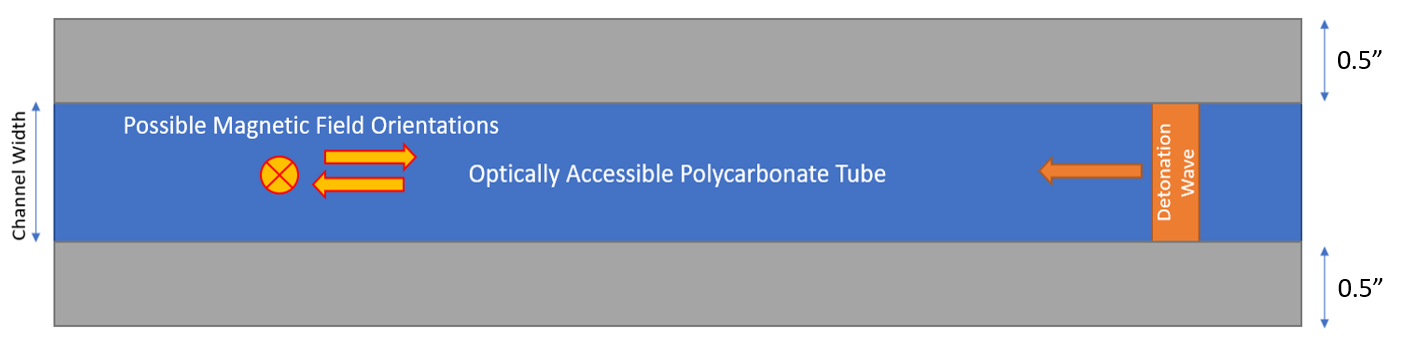
\includegraphics[width=\textwidth]{DetTube.PNG}
        Figure 1: Experimental Setup
    \end{center}
\end{figure}
$$$$
\begin{figure}[h]
    \begin{center}
        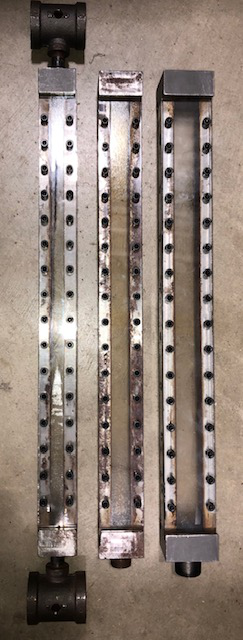
\includegraphics[angle=90, width=\textwidth]{IMG_1044.png}
        \newline Figure 2: Comparison of Tubes
    \end{center}
\end{figure}
\newpage
\indent Figure 3 shows a preliminary calculation of the magnetic field a distance from the magnet, assuming a neodymium bar magnet with dimensions 2 cm by 1 cm by 1 cm.  The magnet will be placed approximately 0.5 inches (the wall thickness) away from the detonation wave, which corresponds to 0.013 meters.  After that point, the magnetic field will have a direct effect on the detonation wave.  It should be noted that this curve is the result of one specific, hypothetical magnet and the values will change based on which magnet is actually used.  In addition, other magnets can be added to the system which could result in a more complex system.  These are all factors that are planned to be altered throughout the project.  
\begin{figure}[h]
    \begin{center}
        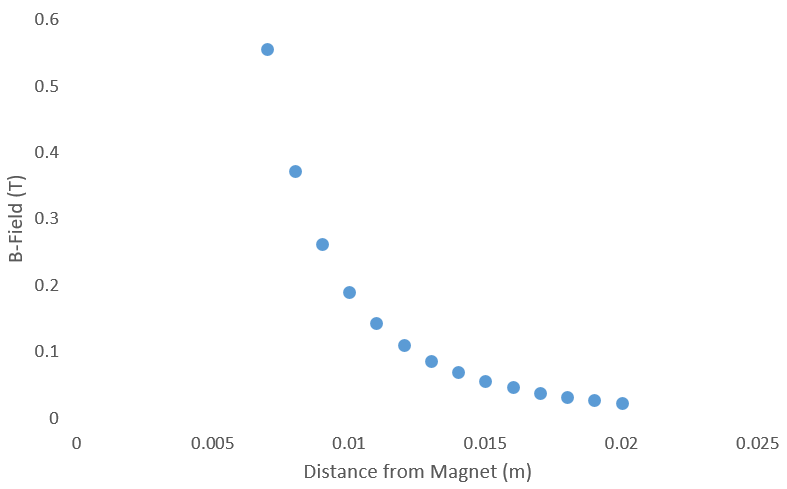
\includegraphics[width=0.75\textwidth]{Bfield.PNG}
        \newline Figure 3: Magnetic Field Simulation
    \end{center}
\end{figure}
\newline
\indent This study will compare the results as various factors are changed.  The magnetic field source can be placed at any point along the tube, and can be oriented so that the Lorentz force direction is either with, against, or across the direction of the detonation wave's propagation.  The source of the magnetic field can either be a permanent magnet or an electromagnet, and the strength of the magnetic field of the two types can be varied by changing the material and size of the magnet or adjusting the flowing current respectively. 
\newline
\indent This study will also examine the effect that varying the channel width will have on the structure of the detonation wave.  While the results of such a change have been studied previously, they did not include the application of an external magnetic field [20].



\begin{center}
    \section*\footnotsize{\textbf{References}}
\end{center}
$$$$
\textbf{1)} Lu, Frank K. "Progress and Challenges in the Development of Detonation Engines for Propulsion and Power Production" \textit{Applied Mechanics and Materials}. Volume 819.  https://www.scientific.net/AMM.819.3.pdf
\newline
\textbf{2)} Cambier, J.L. "Preliminary Modeling for Pulse Detonation Rocket Engine" \textit{35th Joint Propulsion Conference and Exhibit}. https://arc.aiaa.org/doi/10.2514/6.1999-2659
\newline
\textbf{3)} Cambier, J.L. "MHD Augmentation of Pulse Detonation Rocket Engines" \textit{10th AIAA/NAL-NASDA-ISAS International Space Planes and Hypersonic Systems and Technologies Conference}. https://arc.aiaa.org/doi/pdf/10.2514/6.2001-1782
\newline
\textbf{4)} C.   Bruno   and   P.   Czysz,   "An   Electro-Magnetic-Chemical  Hypersonic  Propulsion System", AIAA  98-1582.
\newline
\textbf{5)} Litchford, Ron J., Thompson, Brian, Lineberry, John. "Pulse Detonation MagnetoHydroDynamic Power" \textit{Journal of Propulsion and Power}, Vol. 16 No. 2, 2000
\newline
\textbf{6)} Camier, J. L. "MHD Power Extraction from a Pulse Detonation Engine" AIAA, 1998
\newline
\textbf{7)} Schulz, J.C., Gottiparthi, K.C. & Menon, S. Shock Waves (2012) 22: 579. \newline https://doi.org/10.1007/s00193-012-0412-9
\newline
\textbf{8)} \textit{Magnetohydrodynamics}, mysite.du.edu/~jcalvert/phys/mhd.htm. 
\newline
\textbf{9)} Barmin, A.A. & Lebedeva, L.N. Fluid Dyn (1975) 10: 952. \newline https://doi.org/10.1007/BF01023274
\newline
\textbf{10)} Grigorenko, V.L. & Levin, V.A. Fluid Dyn (1975) 10: 802. \newline https://doi.org/10.1007/BF01015454
\newline
\textbf{11)} Kelly, J.R., Toong, T.V. "Detonation Wave in Electromagnetic Field" \textit{Symposium (International) on Combustion}, pp. 657-664, 1967
\newline
\textbf{12)}Aghajani, Asadolah; Razani, Abdolrahman. Detonation waves in a transverse magnetic field. Michigan Math. J. 53 (2005), no. 3, 647--664. doi:10.1307/mmj/1133894171. https://projecteuclid.org/euclid.mmj/1133894171
\newline
\textbf{13)}Kuznetsov, A.P. & Pleshanov, A.S. Combust Explos Shock Waves (1974) 10: 708. \newline https://doi.org/10.1007/BF01463992
\newline
\textbf{14)}https://search.proquest.com/docview/302381585?accountid=2909&pq-origsite=summon
\newline
\textbf{15)}Kennedy, L.A. Journal of Applied Mathematics and Physics (ZAMP) (1968) 19: 600. https://doi.org/10.1007/BF01594967
\newline
\textbf{16)} Litchford, Ron, Bryan Thompson, and John Lineberry. "Pulse Detonation MHD Experiments."
\newline
\textbf{17)} Griffiths, David J. \textit{Introduction to Electrodynamics}. 4th ed., Cambridge University Press, 2018.
\newline
\textbf{18)}Austin, J. Pingen, F. Shephard, J. "Lead Shock Oscillation and Decoupling in Propagating Detonation" \textit{AIAA}, 2005
\newline
\textbf{19)} Hardeo M. Chin, Hardeo M., Cuppoletti, Daniel R. Obrello, Timothy, Ahmed, Kareem A. "Time-resolved Measurements of Detonation Decoupling and Amplification" \textit{AIAA}, 2020
\newline
\textbf{20)} Katta, Viswanath R., et al. “Effect of Increasing Channel Width on the Structure of Rotating Detonation Wave.” \textit{Proceedings of the Combustion Institute}, Elsevier, 28 June 2018, www.sciencedirect.com/science/article/pii/S1540748918300737. 
\end{document}
